\chapter{Autonomous Load Balancing in a Distributed Hash Table}
\label{chapter:auto-balance}




%http://michiel.buddingh.eu/distribution-of-hash-values

\section{Introduction}

%\subsection{2-4 sentences telling people what you will talk about in the paper}

%\subsection{What are DHTs}
Distributed Hash Tables (DHTs) are a class of well researched decentralized key-value storage systems.
DHTs are most frequently used to construct the overlays of P2P file-sharing systems, such as the incredibly popular BitTorrent \cite{bittorrent}.
DHTs have also been used in many unorthodox applications, such as machine learning \cite{liparameter} and, most relevant for our discussion, distributed computing \cite{chordreduce}.

Our previous research \cite{chordreduce} examined using a DHT as the organizing mechanism for a distributed platform.
This enabled us to create an exceptionally fault tolerant distributed computing platform that was easy to setup and could be run in a completely decentralized P2P environment.

% Copy into disseration start here
%\subsection{What is the significance of the hash function }
One of key components of a Distributed Hash Table is a cryptographic hash function, most commonly SHA1 \cite{sha1}.
Distributed Hash Tables rely on this cryptographic hash function to generate identifiers for data stored on the network.
The cryptographic hash of the filename or other identifier for the data is used as the location of the file or data in the network.
It can also be used to generate the identifiers for nodes in the network.

Ideally, inputing random numbers into a cryptographic hash function should produce a uniformly distributed output.
However, this is impossible in practice \cite{hash-outputs} \cite{thomsen2005cryptographic}.

In practice, that means given any DHT with files and nodes, there will be an inherent imbalance in the network.
Some nodes will end up with a lion's share of the keys, while other will have few responsibilities (Table \ref{tab:medianLoads}).


This makes it especially disheartening to try and ensure as even a load as possible.
We cannot rely on a centralized strategy to fix this imbalance, since that would violate the principles and objects behind creating a fully decentralized and distributed system.

Therefore, if we want to create strategies to act against the inequity of the load distribution, we need a strategy that individual nodes can act upon autonomously.
These strategies need to make decisions that a node can make at a local level, using only information about their own load and the topology they can see.


\subsection{Motivation}
The primary motivation for us is creating a new viable type of platform for distributed computing.
Most distributed computing paradigms, such as Hadoop \cite{hadoop}, assume that the computations occur in a centralized environments.
One enormous benefit is a centralized system has much greater control in ensuring load-balancing.

However, in an increasingly global world where computation is king and the Internet is increasingly an integral part of everyday life, single points of failure failures quickly become more and more risky.
Users expect their apps to work regardless of any power outage affecting an entire region.
Customers expect their services to still be provided regardless of any.
The next big quake affecting the the San Andreas fault line is a matter of when, not if.
Thus, centralized systems with single points of failure become a riskier option and decentralized, distributed systems the safer choice.


Our previous work in ChordReduce \cite{chordreduce} focused on creating a decentralized distributed computing framework based off of the Chord Distributed Hash Table (DHT) and MapReduce.
ChordReduce can be thought of a more generalized implementation of the concepts of MapReduce.
One of the advantages of ChordReduce can be used in either a traditional datacenter or P2P environment.\footnote{The other one being that new nodes could join during runtime and receive work from nodes doing computations.}
Chord (and all DHTs) have the qualities we desire for distributed computing: scalability, fault tolerance, and load-balancing.

Fault tolerance is of particular importance to DHTs, since their primary use case is P2P file-sharing, such as BitTorrent \cite{bittorrent}.
These systems experience high levels of churn-- disruptions to the network topology as a result of nodes entering and leaving the network.
ChordReduce had to have the same level of robustness against churn that Chord did, if not better.

During our experiments with ChordReduce, we found that high levels of churn actually made our computations run \textit{faster}.
We hypothesized that the churn was effectively load-balancing the network.

\subsection{Objectives}
This paper serves to prove our hypothesis that churn can load balance a Distributed Hash Table.
We also set out to show that we can use this in a highly controlled manner to greater effect.
We present three strategies that nodes can use to redistribute the workload in the network.
None of these require a centralized organizer.

We also want to show how distributed computing can be performed in a heterogeneous environment.

%\subsection{Summary}

\section{Previous Work}


ChordReduce \cite{chordreduce} is designed as a more abstract framework for MapReduce, able to run on any arbitrary distributed configuration.
ChordReduce leverages the features of distributed hash tables to handle distributed file storage, fault tolerance, and lookup.
We designed ChordReduce to ensure that no single node is a point of failure and that there is no need for any node to coordinate the efforts of other nodes during processing.

\section{How Work Is Distributed in DHTs: A Visual Guide}
%In this section, we display graphs to give a visual representation of how work is distributed in a Chord \cite{chord} network

As we have previously mentioned, many DHTs use a cryptographic hash function to choose keys for nodes and data.
However, no cryptographic hash function can uniformly distribute it's outputs across its range. 

\begin{table}
	\centering
	\caption{The median distribution of tasks (or files) among nodes.  We can see the standard deviation is fairly close to the expected mean workload ($\frac{tasks}{nodes}$). Each row is the average of 100 trials.}
	\begin{tabular}{r r r r}
		Nodes & Tasks & Median Workload & $\sigma$ \\ \hline
		1000 & 100000 & 69.410   &  137.27  \\
		1000 & 500000 & 346.570  &  499.169 \\
		1000 &1000000 & 692.300  &  996.982 \\
		
		5000 & 100000  & 13.810 & 20.477 \\ 
		5000 & 500000  & 69.280 & 100.344 \\ 
		5000 & 1000000 &138.360 & 200.564 \\ 
		
		10000 & 100000 & 7.000   &  10.492 \\
		10000 & 500000 & 34.550  &   50.366 \\
		10000 & 1000000& 69.180  &  100.319 \\
	\end{tabular}
	\label{tab:medianLoads}
\end{table}




\begin{figure}
	\centering
	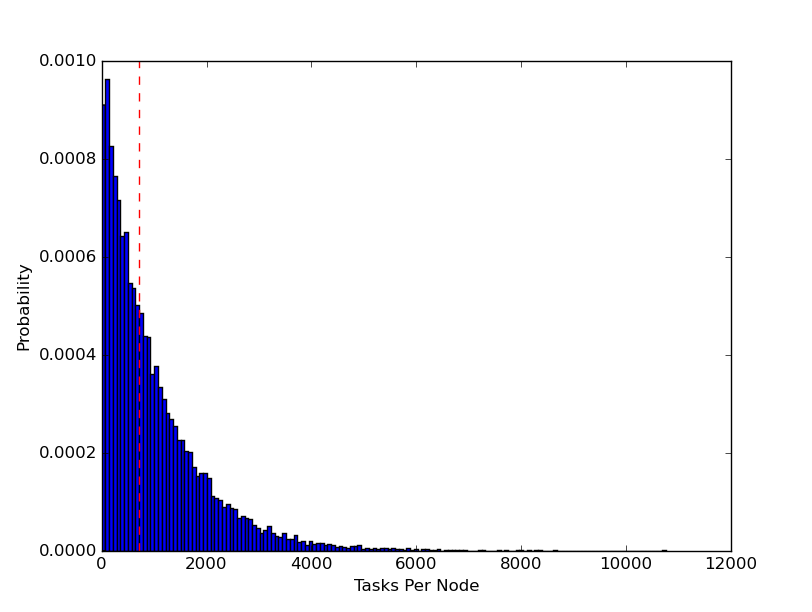
\includegraphics[width=0.7\linewidth]{figs/workloadDistribution}
	\caption[foo]{The probability distribution of workload in a DHT with 1000 nodes and 1,000,000 tasks or files.  The vertical dashed line designates the median.  Keys were generated by feeding random numbers into the SHA1 hash function \cite{sha1}, a favorite for many distributed hash tables.}
	\label{fig:workloadDistribution}
\end{figure}




\section{Simulation}

%We simulate an UrDHT Voronoi based-network in multiple dimensions. \footnote{UrDHT in one dimension is a Chord ring with the definition of responsibility changed to a node being responsible to all data closest to it. A 2-dimensional network will emulate the performance of CAN.}

We assume that the network starts our experiments stable and the data necessary already present on the nodes and backed-up.
The following analysis and simulation relies on an important assumption about DHT behavior often assumed but not necessarily implemented.

We assume that nodes are active and aggressive in creating and monitoring the backups and the data they are responsible for.
Specifically, we will assume it takes  $T_{detect}$ time for a node to detect a change in their responsibility or to detect a new node to hand a backup to and that this check is performed regularly. 
We have demonstrated the effectiveness and viability of implementing an active backup strategy in other work \cite{chordreduce} \cite{urdht}.


Another assumption is that nodes do not have control in choosing their IDs from the range of hash values.

Smaller chunking results in more files spread throughout the  network and a greater chance of the data being evenly spread across the network 

The chances of a critical failure happening within a time interval $ T $ is the chances of some chain or cluster of nodes responsible for a single record dying within $ T $:

$$r^{s}$$

Where $ r $ is the failure rate over that time interval and $s$ is the number nodes storing that record, either as a primary system, or a backup.
Incidentally, this time interval $T = T_{detect} + T_{transfer} $



\subsection{The Parameters}

Our simulations relied on a great number of parameters and variables.
We present each of them below.

\subsubsection{Constants and Terminology}

\begin{description}
	\item [Tick] In a simulation, normal measurements of time such as a second are arbitrary, so we be using the abstract \textit{tick} to measure time.  
	We consider the tick the amount of time it takes a node to complete one task per Sybil and perform the appropriate maintenance.\footnote{If we need to be more concrete, define a tick as a New York Second, which is ``the period of time between the traffic lights turning green and the cab behind you honking.''\\-- Terry Pratchett}
	\item [Maintenance] We assume nodes use the active, aggressive strategy from ChordReduce and  UrDHT \cite{chordreduce} \cite{urdht}.
	Every maintenance cycle, each node checks and updates its list of neighbors (successors and predecessors in Chord) and responds appropriately . 
	We assume that a tick
	\item[Task] A distributed computing job is defined in tasks.
	Each task has a key that corresponds to the key of a file or chunk of a file stored on the network.
	We assume that it takes a tick for a node to consume a task.
	\item [Hash Functions] We will be using SHA-1 \cite{sha1}, a 160-bit hash function.  
	Keys for  will be drawn randomly from this hash function.
\end{description}

\subsubsection{Experimental Variables}
\begin{description}
	\item [Strategy] We use several different strategies (discussed in Section \ref{sec:strategies})  for balancing the load  of tasks among the nodes.
	None of the strategies require centralized data.
	\item [Homogeneity]  This variable controls whether the network is homogeneous or not.
	In a homogeneous network, each node has the same strength, which dictates how much work is consumed per a tick and how many Sybils it can create.
	In a heterogeneous network, each node has a strength chosen uniformly at random from 1 to \texttt{maxSybils}.
	\item [Work Measurement] This variable dictates how much work is consumed in a tick.
	Nodes each consume a single task per a tick or their strength's worth of tasks per a tick.
	\item [Network Size]  How many nodes start in the network.  
	We assume that this can grow during the experiment, either via churn or by creating Sybils.
	\item [Number of Tasks] We measure the size of of a job in tasks.
	This number is typically a few orders of magnitude greater than the network size.
	\item [Churn Rate] Measured in ticks, this can be self induced or a result of actual turbulence in the network.
	Like most analyses of churn \cite{marozzo2012p2p}, we assume churn is constant throughout the experiment and that the joining and leaving rate are equal.
	\item [Max Sybils] \texttt{maxSybils} is the maximum number of Sybils a node can create.
	\item [Sybil Threshold] The \texttt{sybilThreshold} calculates the amount of tasks a node must have before it can create a Sybil.
	\item [Successors] The number of successors each node keeps track of.  
	Nodes also keep track of the same number of predecessors.
	
\end{description}

We also considered using a variable noted as the \texttt{AdaptationRate}, which was the interval at which nodes decided whether or not to create a Sybil.
Preliminary experiments  showed \texttt{AdaptationRate} to have a minimal effect on the runtime, so it was removed.

\subsubsection{Outputs}
The most important output was the number of ticks it took for the experiment to complete.
We compared this runtime to the what we call the ``ideal runtime,'' which is our expected runtime if the every node in the network was given an equal number of tasks and performed them without any churn or creating any Sybils.
For example, consider a network with 1,000 nodes and 100,000 tasks, where each node consumes a single task each tick. 
This network has an ideal runtime of 100 ticks ($ \frac{100000}{1000} = 100$).\footnote{The ideal runtime also happens to be the average number of tasks per node. An interesting, but mathematically unsurprising, coincidence with a few consequences for our data collection.} 

We used these to calculate a ``runtime factor,'' the ratio of the experimental runtime compared to the ideal runtime.
For example, in the network from our previous example took 852 ticks to finish, its factor is 8.52.
We prefer to use this runtime factor for comparisons since it allows us to compare networks of different compositions, task assignments, and other variables.

We also collected data on the average work per tick,


We also ran load-balancing over the first couple steps.
\section{Strategies}
\label{sec:strategies}

For our analysis, we examined four different strategies for nodes to perform autonomous load balancing.
We first show the effects of churn on the speed of a distributed computation.
We then look a three different strategies for in which nodes take a more tactical approach for creating churn and affecting the runtime.

Specifically, nodes perform a limited and controlled Sybil attack \cite{sybil} on their own network in an effort to acquire work with their virtual nodes.
Our strategies dictate when and where these Sybil nodes are created.

We discuss the effectiveness of each of the strategies in Section \ref{sec:autonomous-results} and present results .... .



\subsection{Induced Churn}
Our first strategy, \textit{Induced Churn}, relies solely on churn to perform load balancing.
This churn can either be a product of normal network activity or self-induced.\footnote{All distributed systems experience churn, even if only as hardware failures.}
By self-induced churn, we mean that each node generates a random floating point number between 0 and 1.
If the number is $\leq churnRate$, the node shuts down and leaves the network.

Similarly, we have a pool of waiting nodes the same size as the network.
When they generate an appropriate random number, they join the network.
We assume that nodes enter and leave the network at the same rate.


As we have previously discussed, nodes in our network model actively back up their data and tasks to the a number of successors in case of failure.
In addition, when a node joins, it acquires all the work it is responsible for.
While this model is rarely implemented for DHTs, it is discussed \cite{kademlia} and often assumed to be the way DHTs operate. 
We have implemented it in ChordReduce\cite{chordreduce} and UrDHT\cite{urdht} and demonstrated that the network is capable from recovering from quite catastrophic failures and handling ludicrous amounts of churn.

The consequences of this are that a node suddenly dying is of minimal impact to the network.
This is because a node's successor will quickly detect the loss of the node and know to be responsible for the node's work.
Conversely, a node joining in this model can be a potential boon to the network by joining a portion of the network with a lot of tasks and immediately acquiring work.

This strategy acts as a baseline with which to compare the other strategies, as it is no more than a overcomplicated way of turning machines off and on again. 


\subsection{Random Sybil Injection}
Our second strategy we dubbed \textit{Random Injection}.
In this strategy, once a node's workload was at or below the \texttt{sybilThreshold}, the node would attempt to acquire more work by creating a Sybil node at a random address.

A node checks its threshold and decides whether or not to make a Sybil every 5 ticks.
A node cam also have multiple Sybils, up to \texttt{maxSybils} in a homogeneous network or the node's \texttt{strength} in a heterogeneous network.\footnote{No benefit was shown by increasing \texttt{maxSybils} beyond 10.}
If a node has at least one Sybil, but no work, it has its Sybils quit the network.
We have the decision to make a Sybil occur every 5 ticks and limit each node to creating a single Sybil a check to avoid overwhelming the network.

As we discuss in Section \ref{sec:autonomous-results}, this strategy is surprisingly effective and comes close to ideal runtimes.


\subsection{Neighbor Injection}
\textit{Neighbor Injection} also creates Sybils, but in this case, nodes act on a more restricted range in an attempt to limit the network traffic.
Nodes with \texttt{sybilThreshold} or less tasks attempt to acquire more work by placing a Sybil among it's successors.
Specifically, it looks for the biggest range among it's successors and creates a Sybil in that range.

This range strategy of finding the largest range and injecting assumes that the node with the largest range of responsibility will have been allocated the most work.
This is a sensible assumption since the larger the range of a node's responsibility, the more \textit{potential} tasks it can receive. 
We compare this estimation strategy to actually querying the neighbor and asking how many tasks they have.
An estimation, if accurate, would be preferable to querying the nodes as an estimation can be done without any communication with the successor nodes.

To avoid constant spamming of a range, once a node creates a Sybil, but does not acquire work, it may be advisable to mark that range as invalid for Sybil nodes so nodes don't keep trying the same range repeatedly. 


\subsection{Invitation}
The \textit{Invitation }strategy is the reverse of the Sybil injection strategies.
In  this strategy, nodes with a higher than desired level of work announces it needs help to its predecessors.
The predecessor with least amount of tasks less than the \texttt{sybilThreshold} creates a Sybil to acquire work from the node(it is possible for a call for help to go unanswered).

Nodes determine whether or not they are overburdened using the \texttt{sybilThreshold}.

In invitation, churn losses can be greatly detrimental.

\section{Results Of Experiments}
\label{sec:autonomous-results}

All the raw data can be found online \cite{simulation-data}.

\subsection{Churn}


Our results confirmed our hypothesis from ChordReduce \cite{chordreduce}.
Churn has a profound and significant impact on the network's computation, and this effect is more pronounced with higher rates of churn.
Figure \ref{fig:churnVsTime} plots the runtime of the distributed computation against the level of churn in the network.
This DHT contained 1000 nodes and 100000 tasks.

\begin{figure}
	\centering
	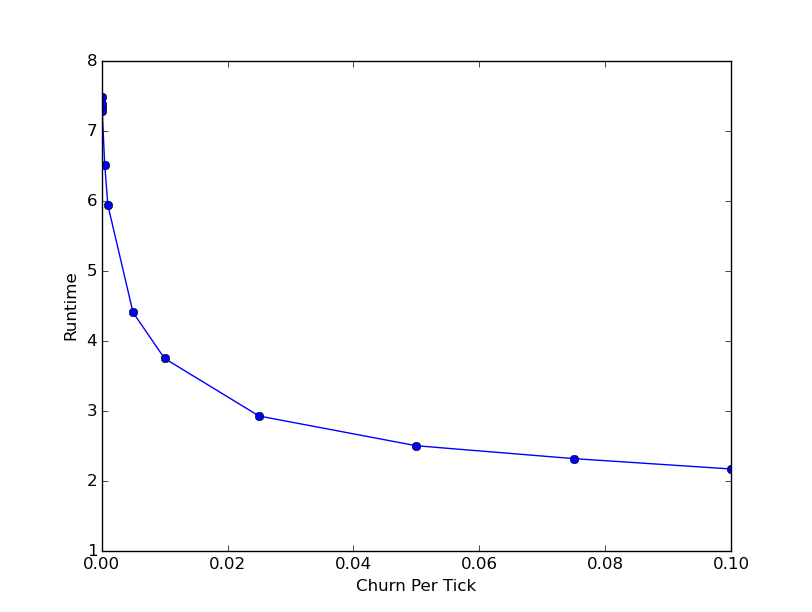
\includegraphics[width=0.7\linewidth]{figs/churnVsTime}
	\caption{This graph shows the effect churn has on runtime in a distributed computation.
		Runtime is measured as how many times slower the computation runs than an ideal computation, where each node receives an equal number of tasks.
		Neither the homogeneity of the network nor work measurement affected the runtime.}
	\label{fig:churnVsTime}
\end{figure}


We note the significantly diminishing returns that occur after a churn rate of 0.01.
One facet not captured by our simulations, but is significant, is the rising maintenance costs after that point.

Also graph average work per tick (Figure \ref{fig:churnVsWork})
\begin{figure}
\centering
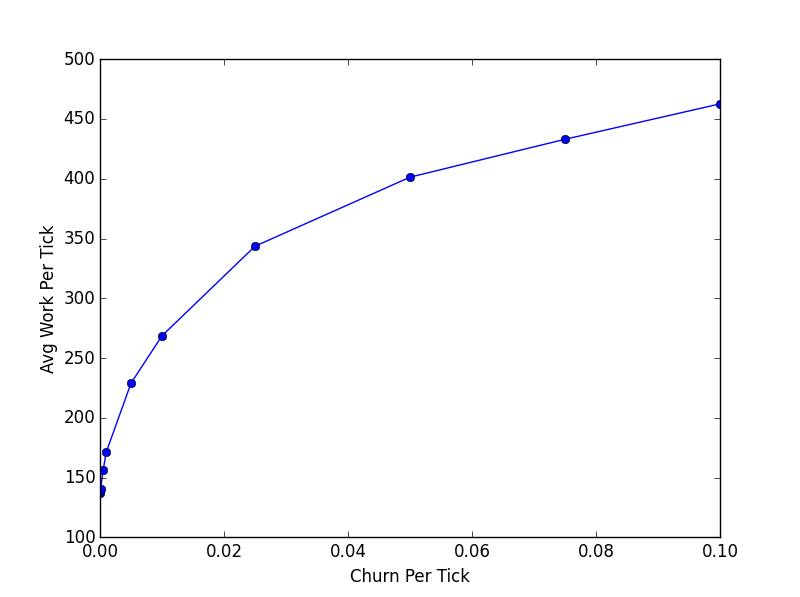
\includegraphics[width=0.7\linewidth]{figs/churnVsWork}
\caption[Churn vs average work per tick]{asd}
\label{fig:churnVsWork}
\end{figure}


\subsection{Random Injection}

The strategy of having under-utilized nodes randomly create Sybil nodes works phenomenally well, approaching very close to the ideal time.


\subsection{Neighbor Injection}

\subsection{Invitation}

